\documentclass[14pt, a4paper]{extarticle}
\usepackage{GOST}
\usepackage{array}
\usepackage{verbatim}
\usepackage[detect-all]{siunitx}
\usepackage{amsmath}
\usepackage{amssymb}
\usepackage[utf8]{inputenc}
\usepackage{hyperref}
\usepackage{tempora}

\makeatletter
\renewcommand\@biblabel[1]{#1.}
\makeatother

\usepackage{listings}
\lstset{ 
	language=Python,
	basicstyle=\small\sffamily, 
	numbers=left, 
	numberstyle=\tiny,
	stepnumber=1,
	numbersep=5pt,
	showspaces=false,            
	showstringspaces=false,      
	showtabs=false,             
	frame=single,            % рисовать рамку вокруг кода
	tabsize=4,      
	commentstyle=\color{green},
	keywordstyle=\color{blue}\textbf,
	numberstyle=\scriptsize\color{gray}, % the style that is used for the line-numbers
	rulecolor=\color{black},
	captionpos=t,
	breaklines=true,         % автоматически переносить строки 
	breakatwhitespace=false, % переносить строки по пробелу
	escapeinside={\#*}{*)} 
}

\begin{document}
	
\begin{table}[ht]
	\centering
	\begin{tabular}{|c|p{400pt}|} 
		\hline
		\begin{tabular}[c]{@{}c@{}} 
\includegraphics[scale=1]{source/b_logo.jpg} \\\end{tabular} &
		\footnotesize\begin{tabular}[c]{@{}c@{}}\textbf{Министерство~науки~и~высшего~образования~Российской~Федерации}\\\textbf{Федеральное~государственное~бюджетное~образовательное~учреждение}\\\textbf{~высшего~образования}\\\textbf{«Московский~государственный~технический~университет}\\\textbf{имени~Н.Э.~Баумана}\\\textbf{(национальный~исследовательский~университет)»}\\\textbf{(МГТУ~им.~Н.Э.~Баумана)}\\\end{tabular}  \\
		\hline
	\end{tabular}
\end{table}
\noindent\rule{\textwidth}{4pt}
\noindent\rule[14pt]{\textwidth}{1pt}
\hfill 
\noindent
\makebox{ФАКУЛЬТЕТ~}%
\makebox[\textwidth][l]{\underline{~«Информатика и системы управления»~~~~~~~~~~~~~~~~~~~~~~~~~~~~~~~~~}}%
\\
\noindent
\makebox{КАФЕДРА~}%
\makebox[\textwidth][l]{\underline{~«Программное обеспечение ЭВМ и информационные технологии»~}}%


\begin{center}
	\vspace{1.5cm}
	{\bf\huge Отчёт\par}
	{\bf\Large по лабораторной работе №4\par}
	\vspace{0.7cm}
\end{center}

\noindent
\makebox{\large{\bf Название:}~~~}
\makebox[\textwidth][l]{\large\underline{Обслуживающий аппарат}}

\noindent
\makebox{\large{\bf Дисциплина:}~~~}
\makebox[\textwidth][l]{\large\underline{~Моделирование~}}\\

\vspace{1.5cm}
\noindent
\begin{tabular}{l c c c c c}
	Студент      & ~ИУ7-75Б~               & \hspace{2.5cm} & \hspace{2cm}                 & &  Д.В. Сусликов \\\cline{2-2}\cline{4-4} \cline{6-6} 
	\hspace{3cm} & {\footnotesize(Группа)} &                & {\footnotesize(Подпись, дата)} & & {\footnotesize(И.О. Фамилия)}
\end{tabular}

\noindent
\begin{tabular}{l c c c c}
	Преподователь & \hspace{5cm}   & \hspace{2cm}                 & & ~~~~~~~И.В. Рудаков~~~~~~~\\\cline{3-3} \cline{5-5} 
	\hspace{3cm}  &                & {\footnotesize(Подпись, дата)} & & {\footnotesize(И.О. Фамилия)}
\end{tabular}

\vspace{0.6cm}
\begin{center}	
	\vfill
	\large \textit {Москва, 2021}
\end{center}

\thispagestyle {empty}
\pagebreak

% ВВЕДЕНИЕ
\clearpage
\section*{Задание}
Необходимо промоделировать систему, состоящую из генератора, памяти, и обслуживающего аппарата. Генератор подает сообщения, распределенные по равномерному закону, они приходят в память и выбираются на обработку по закону из ЛР1 (распределение Пуассона). Количество заявок конечно и задано. Предусмотреть случай, когда обработанная заявка возвращается обратно в очередь. Необходимо определить оптимальную длину очереди, при которой не будет потерянных сообщений. Реализовать двумя способами: используя пошаговый и событийный подходы.

\section*{Теория}
\subsection*{Равномерное распределение}
Функция распределения:
\begin{equation*}
	F_X(x) \equiv P(X \le x) = \left\{
	\begin{matrix}
		0, & x < a \\
		\dfrac{x-a}{b-a}, & a \le x < b \\
		1, & x \ge b
	\end{matrix}
	\right..
\end{equation*}
Функция плотности распределения:
\begin{equation*}
	f_X(x) = \left\{
	\begin{matrix}
		{1 \over b-a}, & x\in [a,b] \\
		0, & x\not\in [a,b]
	\end{matrix}
	\right..
\end{equation*}

\subsection*{Пуассоновское распределение}
Функция распределения:

\begin{equation*}
	F(x) =  \frac{\Gamma(|k + 1), \lambda)}{|k|!}
\end{equation*}

Плотность распределения:

\begin{equation*}
	f(x) = \frac{\lambda^{k}}{k!} e^{-\lambda} 
\end{equation*}	
\newpage

\subsubsection*{Пошаговый подход}
Заключается в последовательном анализе состояний всех блоков системы в момент $t + \Delta t$. Новое состояние определяется в соответствии с их алгоритмическим описанием с учетом действия случайных факторов. В результате этого анализа принимается решение о том, какие системные события должны имитироваться на данный момент времени. Основной недостаток: значительные затраты и опасность пропуска события при больших $\Delta t$.

\subsection*{Событийная модель}
Состояния отдельных устройств изменяются в дискретные моменты времени. При использовании событийного принципа, состояния всех блоков системы анализируются лишь в момент возникновения какого либо события. Момент наступления следующего события, определяется минимальным значением из списка событий.
\newpage
\section*{Результаты работы}
\begin{figure}[h!]
	\centering
	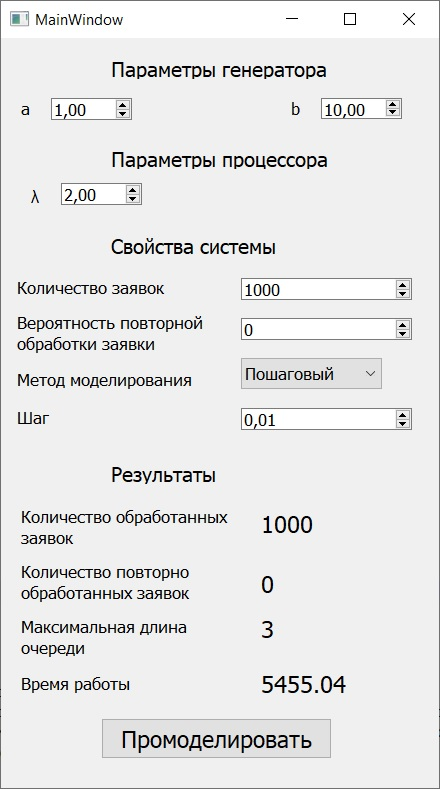
\includegraphics[scale=0.6]{source/step0.jpg}
	\caption{Пошаговый при p = 0}
\end{figure}
\begin{figure}[h!]
	\centering
	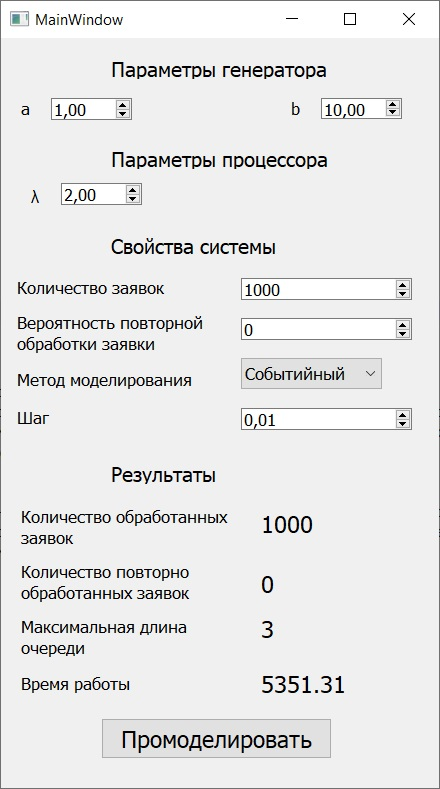
\includegraphics[scale=0.6]{source/event0.jpg}
	\caption{Событийный при p = 0}
\end{figure}
\newpage
\begin{figure}[h!]
	\centering
	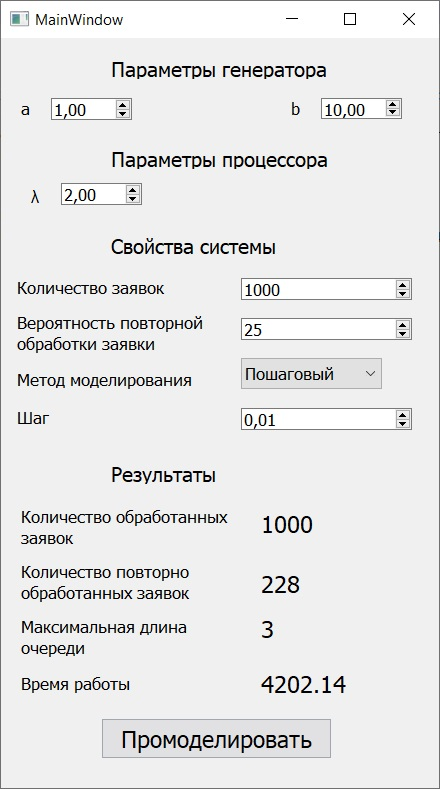
\includegraphics[scale=0.6]{source/step25.jpg}
	\caption{Пошаговый при p = 25}
\end{figure}
\begin{figure}[h!]
	\centering
	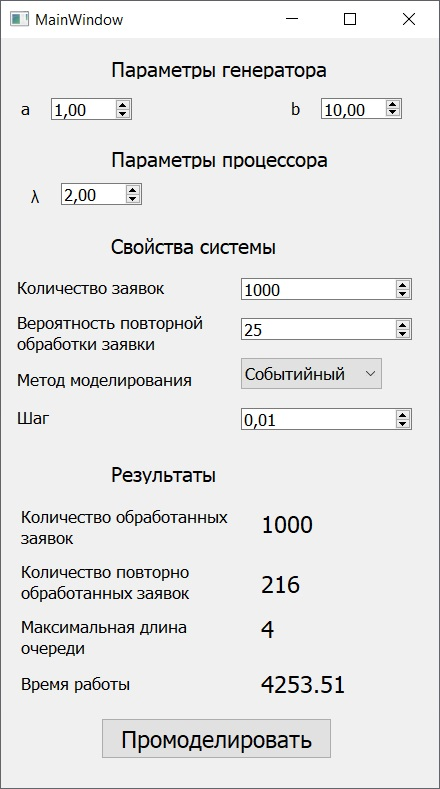
\includegraphics[scale=0.6]{source/event25.jpg}
	\caption{Событийный при p = 25}
\end{figure}
\newpage
\begin{figure}[h!]
	\centering
	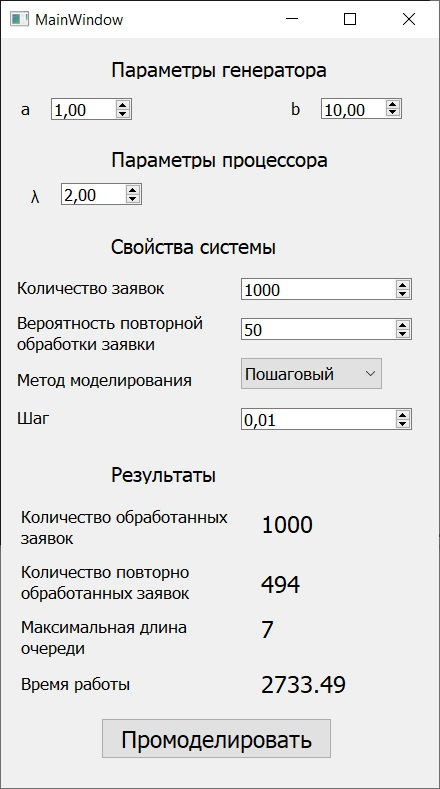
\includegraphics[scale=0.6]{source/step50.jpg}
	\caption{Пошаговый при p = 50}
\end{figure}
\begin{figure}[h!]
	\centering
	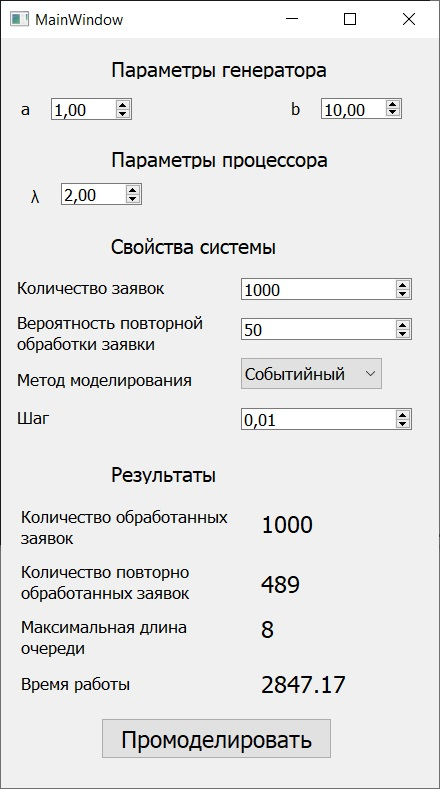
\includegraphics[scale=0.6]{source/event50.jpg}
	\caption{Событийный при p = 50}
\end{figure}
\newpage
\begin{figure}[h!]
	\centering
	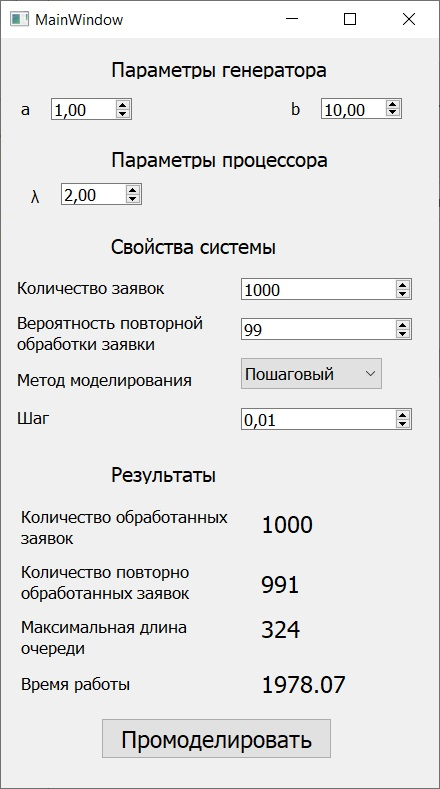
\includegraphics[scale=0.6]{source/step99.jpg}
	\caption{Пошаговый при p = 99}
\end{figure}
\begin{figure}[h!]
	\centering
	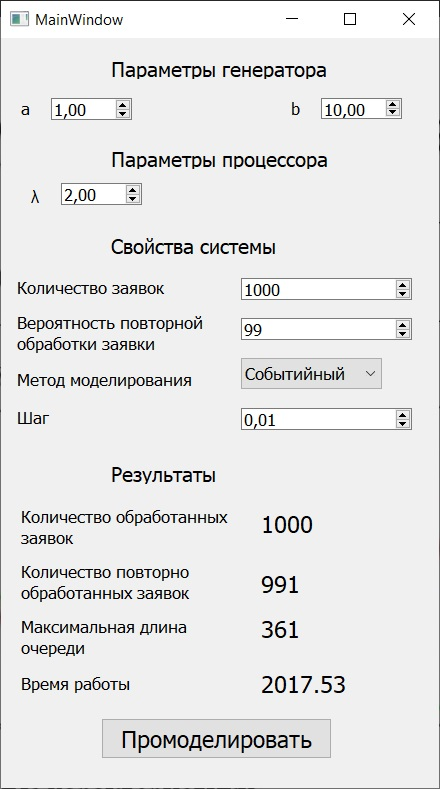
\includegraphics[scale=0.6]{source/event99.jpg}
	\caption{Событийный при p = 99}
\end{figure}

\newpage
\section*{Вывод}
Была смоделирована система, состоящая из генератора, памяти и обслуживающего аппарата.

На выходе получена максимальная длина очереди, число обрабатываемых и повторно обработанных заявок, время обработки.


\section*{Листинг}
\begin{lstlisting}[caption=main.py]
import sys
from PyQt5 import QtWidgets
from PyQt5 import uic, QtWidgets, QtGui
from PyQt5.QtWidgets import QApplication, QWidget, QListWidgetItem,  QTableWidgetItem, QMessageBox
import design
from models import event_model, step_model
from distributions import UniformDistribution, PoissonDistribution

class App(QtWidgets.QMainWindow, design.Ui_MainWindow):
	def __init__(self):
		a, b = 1, 10
		self.generator = UniformDistribution(a, b)
		
		lyambda = 2.0
		self.processor = PoissonDistribution(lyambda)
		
		self.total_tasks = 1000
		self.repeat_percentage = 0
		self.step = 0.01
		
		super().__init__()
		self.setupUi(self)
		self.initUI()
	
	def initUI(self):
		self.startBtn.clicked.connect(self.startBtnPushed)
	
	
	def startBtnPushed(self):
		a = self.aSpinBox.value()
		b = self.bSpinBox.value()
		lyambda = self.lyambdaSpinBox.value()
		
		self.generator = UniformDistribution(a, b)
		self.processor = PoissonDistribution(lyambda)
		
		self.total_tasks = self.tasksSpinBox.value()
		self.repeat_percentage = self.repeatSpinBox.value()
		self.step = self.stepSpinBox.value()
		processed_tasks, reentered_tasks, max_queue_len, t = 0, 0, 0, 0
		if self.methodComboBox.currentText() == "Sobitiyniy":
			processed_tasks, reentered_tasks, max_queue_len, t = event_model(self.generator, self.processor, self.total_tasks, self.repeat_percentage)
		else:
			processed_tasks, reentered_tasks, max_queue_len, t = step_model(self.generator, self.processor, self.total_tasks, self.repeat_percentage)
		
		self.resTasksLabel.setText(str(processed_tasks))
		self.repeatTasksLabel.setText(str(reentered_tasks))
		self.maxLenLabel.setText(str(max_queue_len))
		self.timeLabel.setText(str(round(t, 2)))


def main():
	app = QtWidgets.QApplication(sys.argv)
	window = App()
	window.show()
	app.exec_()
	
	print('event_model:', event_model(generator, processor, total_tasks, repeat_percentage))
	print('step_model:', step_model(generator, processor, total_tasks, repeat_percentage, step))


if __name__ == '__main__':
	main()

\end{lstlisting}

\begin{lstlisting}[caption=models.py]
import random


def step_model(generator, processor, total_tasks=0, repeat=0, step=0.001):
	processed_tasks = 0
	t_curr = step
	t_gen_prev = t_proc = 0
	t_gen = generator.generate()
	t_proc = t_gen + processor.generate()
	cur_queue_len = max_queue_len = 0
	reentered_tasks = 0
	
	while processed_tasks < total_tasks:
	if t_curr > t_gen:
		cur_queue_len += 1
		if cur_queue_len > max_queue_len:
			max_queue_len = cur_queue_len
		t_gen += generator.generate()
	
		if t_curr > t_proc:
			if cur_queue_len > 0:                
				processed_tasks += 1
			if random.randint(1, 100) <= repeat:
				cur_queue_len += 1
				reentered_tasks += 1
			cur_queue_len -= 1
			if cur_queue_len > 0:
				t_proc += processor.generate()
			else:
				t_proc = t_gen + processor.generate()
	t_curr += step
	
	return processed_tasks, reentered_tasks, max_queue_len, t_curr

def event_model(generator, processor, total_tasks=0, repeat=0):
	processed_tasks = 0
	t_gen = generator.generate()
	t_proc = t_gen + processor.generate()
	cur_queue_len = max_queue_len = 0
	reentered_tasks = 0
	while processed_tasks < total_tasks:
		if t_gen <= t_proc:
		cur_queue_len += 1
		if cur_queue_len > max_queue_len:
			max_queue_len = cur_queue_len
		t_gen += generator.generate()
	
	if t_gen >= t_proc:
		if cur_queue_len > 0:                
			processed_tasks += 1
			if random.randint(1, 100) <= repeat:
				cur_queue_len += 1
				reentered_tasks += 1
			cur_queue_len -= 1
			if cur_queue_len > 0:
				t_proc += processor.generate()
			else:
				t_proc = t_gen + processor.generate()
	
	return processed_tasks, reentered_tasks, max_queue_len, t_proc	
\end{lstlisting}

\begin{lstlisting}[caption=distributions.py]
	from numpy.random import uniform, normal, poisson
	import random	
	
	class UniformDistribution:
		def __init__(self, a: float, b: float):
			self.a = a
			self.b = b
		
		def generate(self):
			return uniform(self.a, self.b)
	
	class PoissonDistribution:
		def __init__(self, lyambda):
			self.lyambda = lyambda
	
		def generate(self):
			return poisson(self.lyambda)
	
	class NormalDistribution:
		def __init__(self, mu, sigma):
			self.mu = mu
			self.sigma = sigma
		
		def generate(self):
			return normal(self.mu, self.sigma)
		
\end{lstlisting}

\end{document}









